\documentclass[tikz,border=4pt]{standalone}
\usepackage[T1]{fontenc}
\usepackage{mathptmx}
\usetikzlibrary{arrows.meta,calc,fit}
\begin{document}
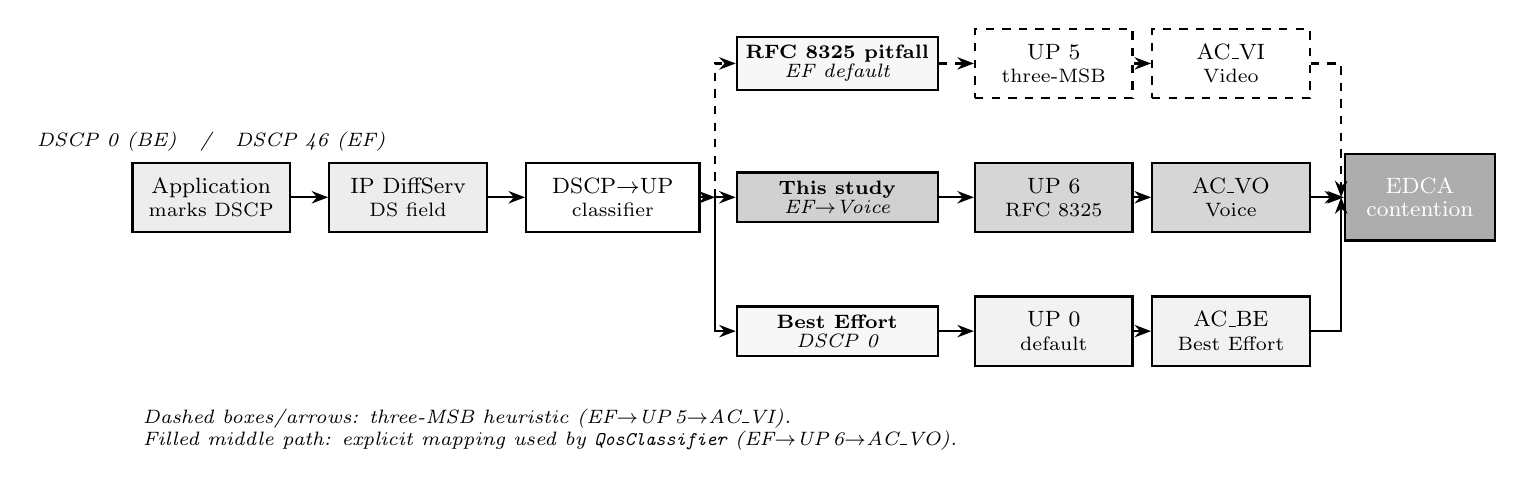
\begin{tikzpicture}[
  font=\footnotesize,
  >=Stealth,
  thick,
  box/.style={draw, thick, align=center, inner sep=4pt, minimum height=0.88cm},
  stage/.style={box, fill=black!7, minimum width=2.00cm},
  clf/.style={box, fill=white, minimum width=2.20cm},
  bad/.style={box, dashed, fill=white, minimum width=2.00cm},
  good/.style={box, fill=black!16, minimum width=2.00cm},
  be/.style={box, fill=black!5, minimum width=2.00cm},
  sink/.style={box, fill=black!32, text=white, minimum width=1.90cm, minimum height=1.10cm},
  callout/.style={draw, thick, align=center, inner sep=3pt, font=\scriptsize\bfseries,
                  minimum width=2.55cm},
  lbl/.style={font=\scriptsize\itshape, align=left},
  arr/.style={-{Stealth[length=2.1mm]}, thick},
]
  % ----- Common trunk -----
  \node[stage] (app) at (0.00,2.50) {Application\\[-1pt]{\scriptsize marks DSCP}};
  \node[stage] (ip)  at (2.50,2.50) {IP DiffServ\\[-1pt]{\scriptsize DS field}};
  \node[clf]   (cl)  at (5.10,2.50) {DSCP$\rightarrow$UP\\[-1pt]{\scriptsize classifier}};

  \node[lbl, anchor=south, align=center] at (app.north)
    {DSCP 0 (BE)\quad/\quad DSCP 46 (EF)};

  \draw[arr] (app) -- (ip);
  \draw[arr] (ip) -- (cl);

  % Split hub
  \coordinate (hub) at (6.40,2.50);
  \draw[arr] (cl.east) -- (hub);

  % ----- Three well-spaced lanes -----
  % y = 4.20 pitfall | 2.50 study | 0.80 BE
  \node[callout, fill=black!3] (cPit) at (7.95,4.20) {RFC 8325 pitfall\\[-1pt]{\normalfont\itshape EF default}};
  \node[bad] (up5) at (10.70,4.20) {UP 5\\[-1pt]{\scriptsize three-MSB}};
  \node[bad] (vi)  at (12.95,4.20) {AC\_VI\\[-1pt]{\scriptsize Video}};

  \node[callout, fill=black!18] (cStu) at (7.95,2.50) {This study\\[-1pt]{\normalfont\itshape EF$\rightarrow$Voice}};
  \node[good] (up6) at (10.70,2.50) {UP 6\\[-1pt]{\scriptsize RFC 8325}};
  \node[good] (vo)  at (12.95,2.50) {AC\_VO\\[-1pt]{\scriptsize Voice}};

  \node[callout, fill=black!3] (cBE) at (7.95,0.80) {Best Effort\\[-1pt]{\normalfont\itshape DSCP 0}};
  \node[be] (up0) at (10.70,0.80) {UP 0\\[-1pt]{\scriptsize default}};
  \node[be] (acbe) at (12.95,0.80) {AC\_BE\\[-1pt]{\scriptsize Best Effort}};

  % Hub → callouts → UP → AC
  \draw[arr, dashed] (hub) |- (cPit.west);
  \draw[arr]         (hub) -- (cStu.west);
  \draw[arr]         (hub) |- (cBE.west);

  \draw[arr, dashed] (cPit) -- (up5);
  \draw[arr, dashed] (up5) -- (vi);

  \draw[arr] (cStu) -- (up6);
  \draw[arr] (up6) -- (vo);

  \draw[arr] (cBE) -- (up0);
  \draw[arr] (up0) -- (acbe);

  % ----- Merge to contention -----
  \node[sink] (tx) at (15.35,2.50) {EDCA\\[-1pt]contention};
  \coordinate (merge) at (14.35,2.50);
  \draw[arr, dashed] (vi.east) -| (merge);
  \draw[arr] (vo.east) -- (merge);
  \draw[arr] (acbe.east) -| (merge);
  \draw[arr] (merge) -- (tx.west);

  % ----- Legend -----
  \node[lbl, anchor=west] at (-1.0,-0.45) {%
    Dashed boxes/arrows: three-MSB heuristic (EF$\rightarrow$UP\,5$\rightarrow$AC\_VI).\\
    Filled middle path: explicit mapping used by \texttt{QosClassifier}
    (EF$\rightarrow$UP\,6$\rightarrow$AC\_VO).};
\end{tikzpicture}
\end{document}
